\begin{filecontents*}{example.eps}
%!PS-Adobe-3.0 EPSF-3.0
%%BoundingBox: 19 19 221 221
%%CreationDate: Mon Sep 29 1997
%%Creator: programmed by hand (JK)
%%EndComments
gsave
newpath
  20 20 moveto
  20 220 lineto
  220 220 lineto
  220 20 lineto
closepath
2 setlinewidth
gsave
  .4 setgray fill
grestore
stroke
grestore
\end{filecontents*}
%
\RequirePackage{fix-cm}
\documentclass[smallextended,twocolumn]{svjour3}
%
\smartqed  % flush right qed marks, e.g. at end of proof
%
\usepackage{graphicx}
\usepackage{float}
\usepackage{amsmath}
\usepackage{mathtools}
\begin{document}
\title{A Personalized Photo Enhancement Agent}

\author{Jason Tellis         \and
        Ling Ouyang	\and Mugdha Jain %etc.
}

\institute{M. Jain \at
              \email{mugdha.jain@sjsu.edu}           
           \and
           L. Ouyang \at
              \email{ling.ouyang@sjsu.edu}
           \and
            J. Tellis \at
            \email{prashanthjason.tellis@sjsu.edu}
}

\date{Received: date / Accepted: date}
% The correct dates will be entered by the editor

\maketitle

\begin{abstract}
An intelligent agent incorporating user's personal preference and feedback was developed for personalized photo enhancement. Most image enhancement techniques rely on heuristic algorithms with some static or probabilistic parameters. This agent learns the user's latent aesthetic preferences from their past images. Using this knowledge, it enhances and customizes new images to match the user's taste. 
The model was trained on user-clicked pictures and user provided labels such as 'liked' and 'disliked'. The agent learns from the training dataset and applies this to improve the user's new photos such that the image quality and style is tailored to the user's personal taste.
To evaluate the performance, users were given a blind test to decide which they liked more between the original and the enhanced photo. 
The images mostly focus on having a human subject.

\keywords{Image Classification \and Image Enhancement}

\end{abstract}

\section{Introduction}
In this era of being connected to everyone through our mobile devices, sharing photos has become an important form of communication. Everyone wants to look their best in photos to get the most attention from their social circle. Hence, photo enhancement plays an important role in our lives. In this project, we were interested in discovering how intuitive aesthetics of an image could be modeled to enhance photos instead of relying on heuristic/probabilistic approaches.  

\subsection{Related Work}
A lot of research effort has gone into investigating how latent aesthetic features can be used to enhance images. A photo editing system, Creatism, that mimics landscape photographer's workflow to produce enhanced photos \cite{DBLP:journals/corr/FangZ17} was recently introduced by Google researchers. Another group \cite{DBLP:journals/corr/ChenKSCM17}  exploited professional photographs from the web to train their aesthetics model by examining pairs of views without having to apply any explicit photographic rules. 

\section{Materials \& Methods}
\begin{figure}[!h]
  \includegraphics[scale=0.4]{AgentDesign.png}
\caption{High Level Design of the Agent}
\label{fig:1}       
\end{figure}
\label{sec:1}
\subsection{Environment}
\label{sec:2}
The Environment class operated on a set of images captured by users under various lighting conditions (sunny, daylight, twilight, night), scene types (portrait, landscape) and locations (indoor and outdoor). 
It presented the labelled images in the training set to the agent to build a model for classification.
 %(see Sect.~\ref{sec:1}).
\subsection{Sensor} 
The sensor module passed the percepts to the agent function. The user interface for the sensor allows the user to select a folder of images for training the classifier.
\subsection{Percepts}
The percepts are the images to be classified and enhanced by the agent. Examples of good and bad images are shown in Fig 2-3.
\begin{figure}[!h]
  \includegraphics[scale=0.20]{Farewell_Original.jpg}
\caption{Sample Good Image}
\label{fig:2} 
\end{figure}

\begin{figure}[!h]
  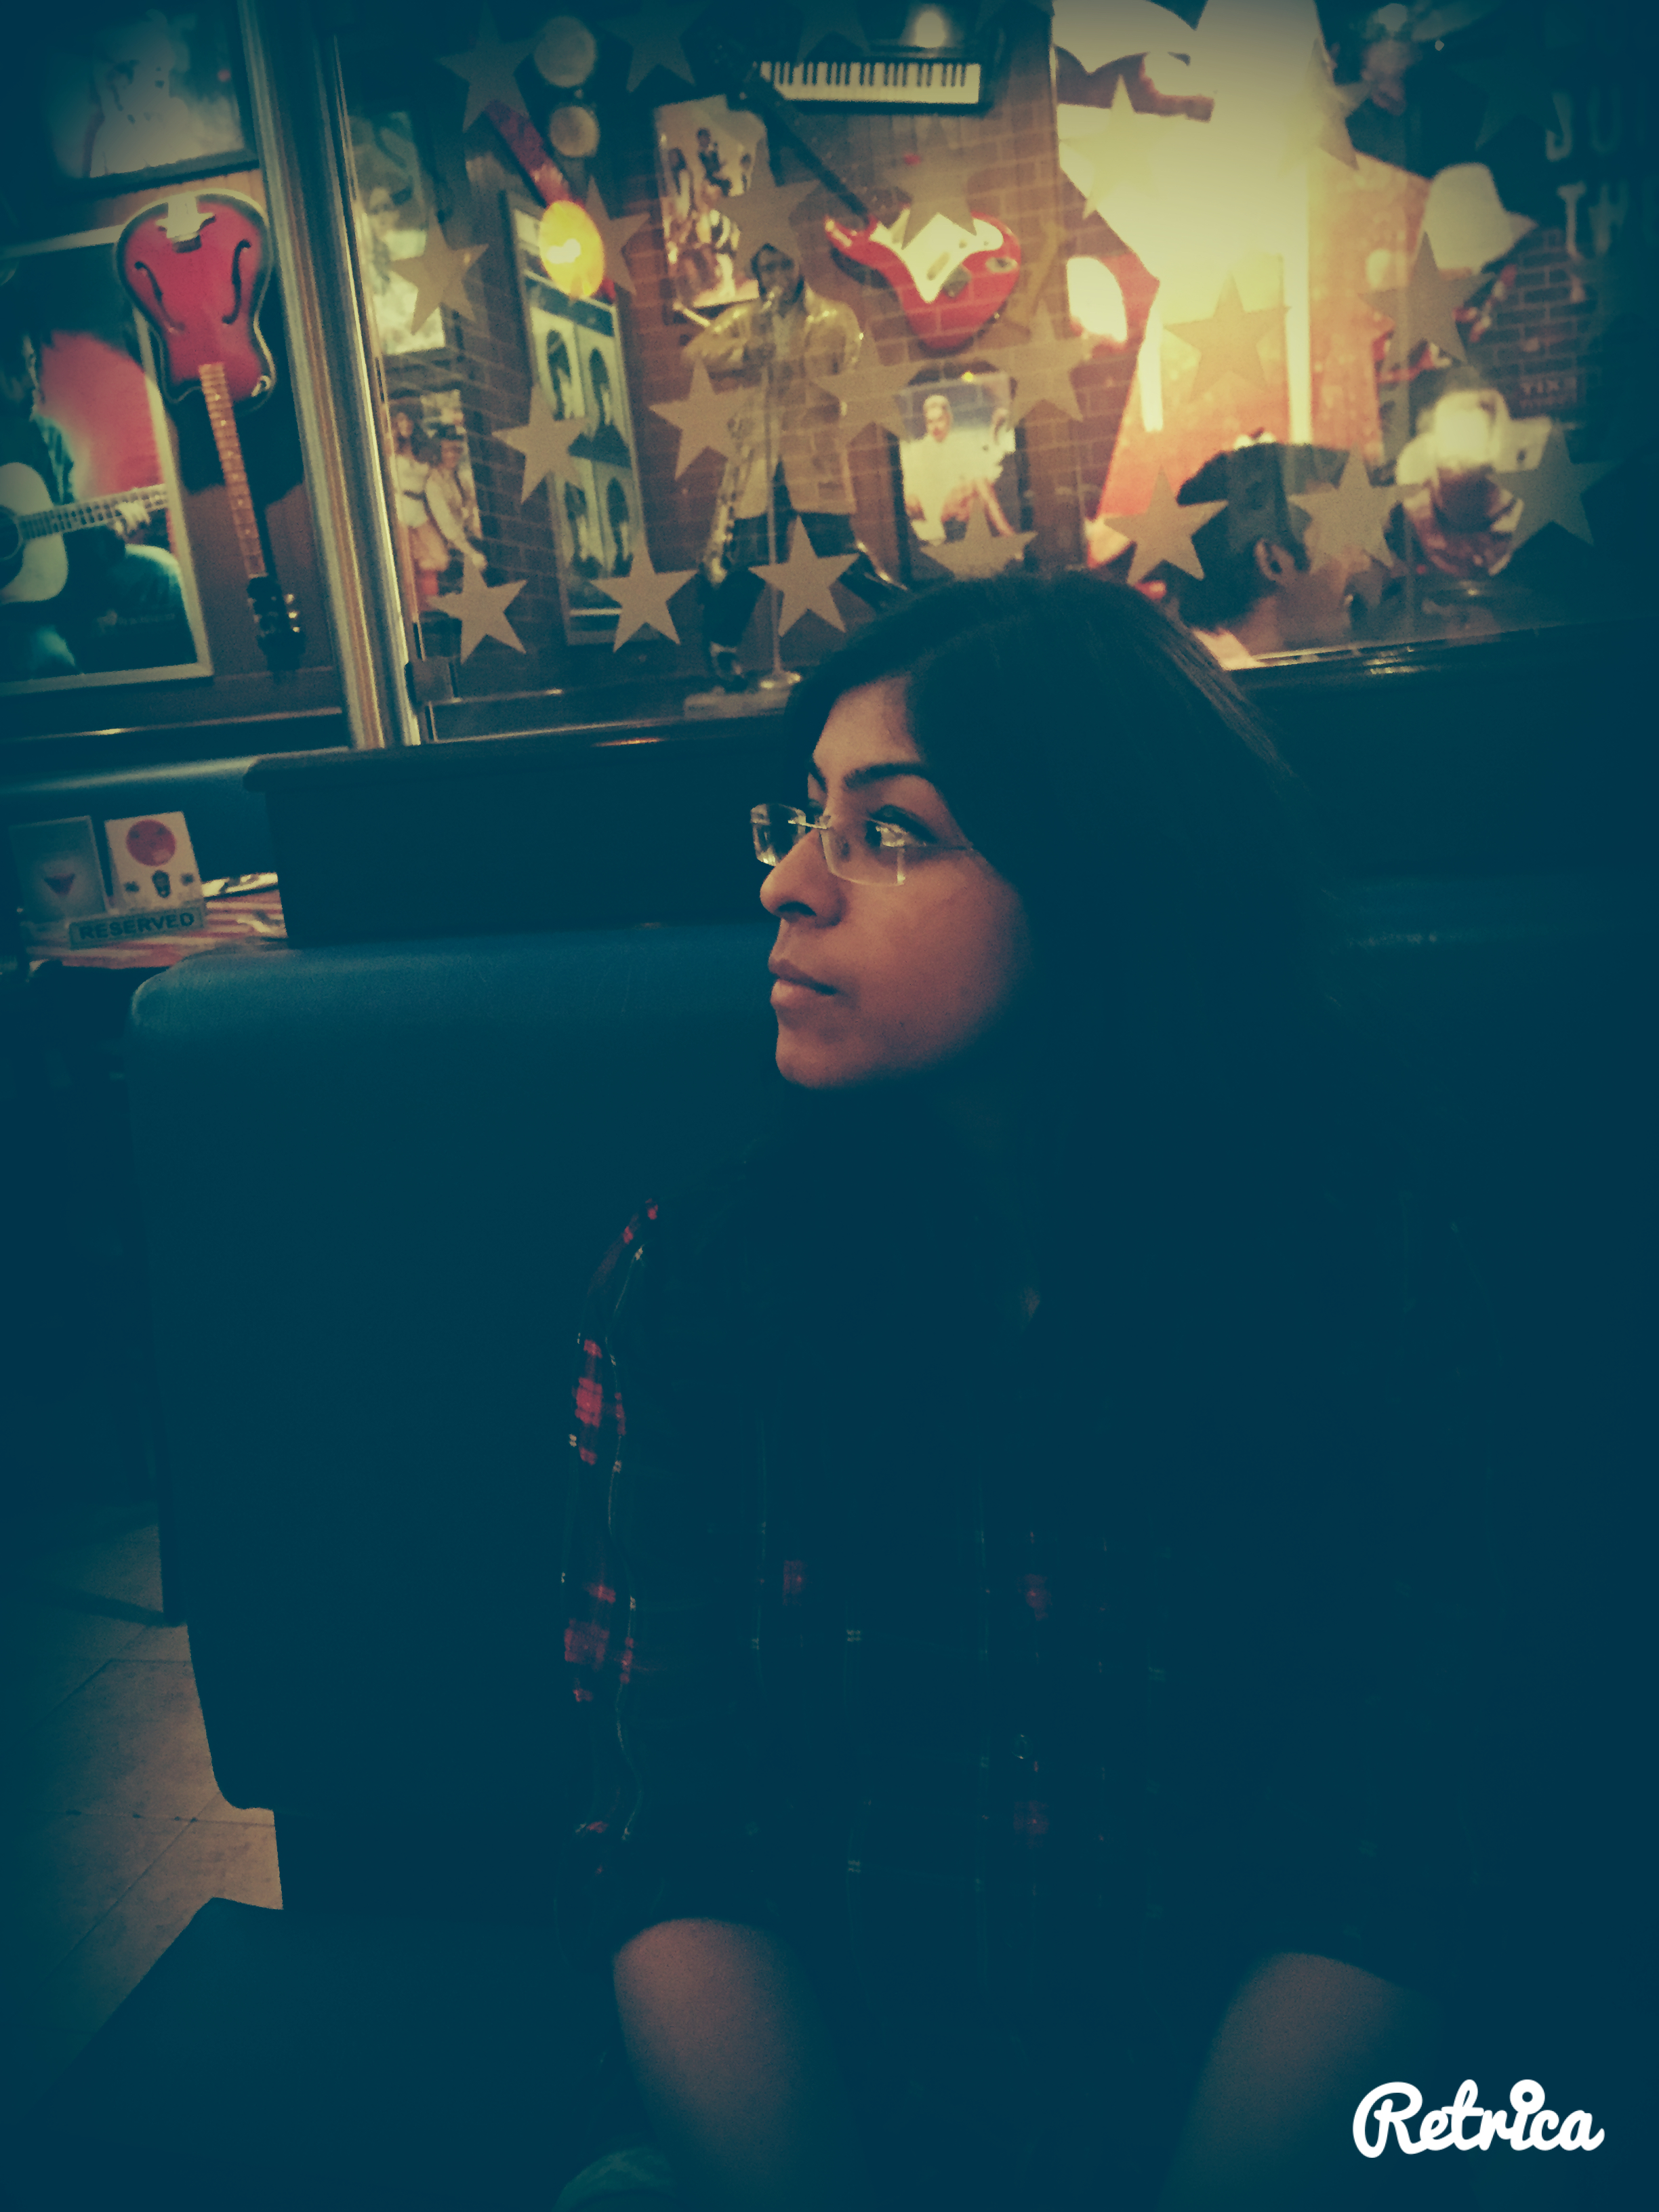
\includegraphics[scale=0.08]{TGIF_Original.jpg}
\caption{Bad Image}
\label{fig:3}       
\end{figure}

\subsection{Agent Function}
The 3 tasks that the agent function performs are:
\begin{enumerate}
	\item Feature Extraction
	\item Image Classification
	\item Enhancement of Images
\end{enumerate}

\subsubsection{Image Feature Extraction}
Feature extraction was performed to retrieve meaningful information so that the agent learned what a good photo should look like. The following 7 features were used:
\begin{enumerate}
  \item Number of Faces
  \item Skin Probability: Possibility of each pixel being skin
  \item Skin Colour
  \item Face Sharpness
  \item Face Smoothness
   \item Image Entropy(Contrast and Brightness)
  \item Global Edge Sharpness
 \end{enumerate}

\subsubsection{Classifier}
The classifier classifies a percept as good or bad depending on the classification model used(k-NN, SVM and Random Forest). The images classified as bad were sent to the enhancer module to be modified.
\subsubsection{Enhancer}
A bad image is enhanced based on specific enhancement criteria that is calculated by taking the average feature vector of all the good images in the training data set at each iteration.
\subsection{Actuator}
The actuator displayed all the processed images (un-enhanced and enhanced) to the user and recorded their feedback. Finally the images that the user tagged as good were sent back into the training dataset to be used the next time an image needs to be classified. This allowed the agent to incrementally learn and accumulate the user's preference of good images.
The user interface for the actuator is a window that displays all the processed test images and allows the user to either 'Like' or 'Dislike' the image.
\subsection{Performance Measures}
The performance of the classifier and enhancer was measured separately.
\paragraph{Evaluating the Classifier:} The accuracy of predictions obtained for each new set of images was used to evaluate the classifier.
\paragraph{Evaluating the Enhancer:} The enhanced images are displayed to the user for their feedback. Once the enhanced images are displayed to the user for feedback, the enhancer effectiveness 'e' was calculated using the following formula:\\

\[e= \frac{\splitfrac{w_1(bad\rightarrow good)+w_2(good\rightarrow bad)}{+w_3(bad\rightarrow bad)+w_4(good\rightarrow good)}}{w_1(No. of Test Images)} \]
where:
\begin{description}
\item[$w_1$] = 2
\item[$w_2$] = -2
\item[$w_3$] = -1
\item[$w_4$] = 0
\end{description}
 The working principle is to keep a count of whether the enhancements are liked by the user as shown in the Table:

\begin{table}[H]
% table caption is above the table
\caption{Evaluation Parameters for Enhancer}
\label{tab:1}       % Give a unique label
% For LaTeX tables use
\begin{tabular}{lll}
\hline\noalign{\smallskip}
Classification Label & Enhanced Image Label & Weight  \\
\noalign{\smallskip}\hline\noalign{\smallskip}
Bad & Good & 2 \\
Good & Bad & -2 \\
Bad & Bad & -1 \\
Good & Good & 0 \\
\noalign{\smallskip}\hline
\end{tabular}
\end{table}
The weighted sum of these parameters is normalized by dividing it by the number of test images to obtain a value between -1 and 1. Thus, a more positive score indicates that the enhancer performed well and a more negative score implies that the enhancer did not do well.




\section{Experiments}
\subsection{Training Data Set}
A training data set of 40 images per user was built manually and labelled 'good' or 'bad' based on the user's personal taste.
\subsection{Validation Data Set}
Validation data set was built using cross validation of the images in the training data set. 
\subsection{Test Data Set}
To assess the performance of our agent, new images of the user were obtained.



\section{Results} 
\subsection{k Nearest Neighbors}
The k Nearest Neighbors classifier produced the following confusion matrix for k=5 with an accuracy of 90.32\%.
% For tables use
\begin{table}[H]
% table caption is above the table
\caption{Confusion Matrix for kNN}
\label{tab:1}       % Give a unique label
% For LaTeX tables use
\begin{tabular}{lll}
\hline\noalign{\smallskip}
Class & Predicted Good & Predicted Bad  \\
\noalign{\smallskip}\hline\noalign{\smallskip}
Actual Good & 24 & 1 \\
Actual Bad & 2 & 4 \\
\noalign{\smallskip}\hline
\end{tabular}
\end{table}


\subsection{SVM}
The Support Vector Machine Classifier produced the following confusion matrix for linear kernel with an accuracy of 87.10\%.
% For tables use
\begin{table}[H]
% table caption is above the table
\caption{Confusion Matrix for SVM}
\label{tab:1}       % Give a unique label
% For LaTeX tables use
\begin{tabular}{lll}
\hline\noalign{\smallskip}
Class & Predicted Good & Predicted bad  \\
\noalign{\smallskip}\hline\noalign{\smallskip}
Actual Good & 24 & 1 \\
Actual Bad & 3 & 3 \\
\noalign{\smallskip}\hline
\end{tabular}
\end{table}

\subsection{Random Forest}
The Random Forest Classifier produced the following confusion matrix for 10 trees with an accuracy of 67.74\%.
% For tables use
\begin{table}[H]
% table caption is above the table
\caption{Confusion Matrix for Random Forest}
\label{tab:1}       % Give a unique label
% For LaTeX tables use
\begin{tabular}{lll}
\hline\noalign{\smallskip}
Class & Predicted Good & Predicted bad  \\
\noalign{\smallskip}\hline\noalign{\smallskip}
Actual Good & 19 & 6 \\
Actual Bad & 4 & 2 \\
\noalign{\smallskip}\hline
\end{tabular}
\end{table}

\subsection{Enhancer Results}
The following images demonstrate the enhanced image against the original image.
\begin{figure}[!h]
  \includegraphics[scale=0.07]{party_foggy_dark.jpg}
\caption{Original Image}
\label{fig:3}       
\end{figure}

\begin{figure}[!h]
  \includegraphics[scale=0.07]{party_foggy_dark-Enhanced.jpg}
\caption{Enhanced Image}
\label{fig:3}       
\end{figure}

\begin{figure}[!h]
  \includegraphics[scale=0.20,angle=-90,origin=c]{Mugdha_sitting_original.jpg}
\caption{Original Image}
\label{fig:3}       
\end{figure}

\begin{figure}[!h]
  \includegraphics[scale=0.20]{Mugdha_sitting_enhanced.jpg}
\caption{Enhanced Image}
\label{fig:3}       
\end{figure}
There is a clear distinction between the enhanced and original image. For Fig. 4-5, the overall sharpness of the image and the skin tone has been enhanced. For Fig.6-7, the face has been brightened and smoothed and the global contrast has been enhanced.


 
The enhancer is evaluated by calculating how effective its enhancements were on a test data set of 31 images.
\begin{table}[H]
% table caption is above the table
\caption{Confusion Matrix for Evaluating the Agent}
\label{tab:1}       % Give a unique label
% For LaTeX tables use
\begin{tabular}{lll}
\hline\noalign{\smallskip}
Class & Predicted Good & Predicted bad  \\
\noalign{\smallskip}\hline\noalign{\smallskip}
User-labelled Good& 0 & 16 \\
User-labelled Bad & 8 & 7 \\
\noalign{\smallskip}\hline
\end{tabular}
\end{table}
The accuracy of the agent was found to be 22.58\%.The effectiveness for this set of test data was found to be -0.5968 indicating that the agent did not do well.


\subsection{Future Work}
The following tasks need to be improved/implemented in the future:
\begin{enumerate}
\item Improve the UI for the agent.
\item Automate fetching images from social media accounts of the user.
\item Feature Engineering to extensively personalize the features extracted for each individual user.
\item Automating annotation of training data by making use of social media metrics.
\end{enumerate}

\bibliography{AIFinalReport} 
\bibliographystyle{spbasic}

\end{document}
% end of file template.tex

